\section{Preliminary Results}
\label{sec:eval}

\begin{figure}
    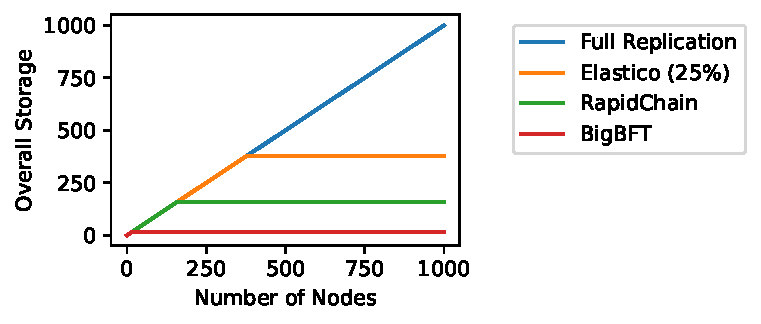
\includegraphics[width=0.95\linewidth]{graphs/redundancy}
    \caption{The overall storage consumption of various works, normalized to the state size.}
    \label{fig:redundancy}
\end{figure}

We conduct a numerical analysis of the total storage consumption across various blockchain designs, and the results are presented in \autoref{fig:redundancy}.
The security parameters for \textsc{Elastico}, RapidChain, and the active layer of \sys are consistently set at $10^{-6}$.
\ifspace
Notice that \sys provides deterministic security guarantees.
Under this setting, the probability of the other works ensuring security is equivalent to the probability of \sys utilizing its fast path.
So this is a fair comparison since the performance of \sys's fast path is on par with the other works.
Also notice that \textsc{Elastico} is plotted with $\frac{1}{4}$ faulty nodes, which is the targeted scenario of its design.
As we discussed in \autoref{sec:bg}, its storage consumption would be equivalent to full replication with $\frac{1}{3}$ faulty nodes.
\fi
The results demonstrate that \sys achieves superior storage scalability.
\sys incurs a storage overhead of at most $16\times$ the state size, irrespective of the number of nodes in the system.
RapidChain and \textsc{Elastico} can also achieve storage scalability but with significantly larger upper bounds on storage overhead ($158\times$ and $378\times$ the state size, respectively).
Thanks to the decomposed design, \sys can start sharding and enjoy scalable storage consumption from almost zero scale.
In the contrary, the processing sharding design disables sharding with committee sizes smaller than hundreds, not even mention that it also compromises the security properties (\autoref{sec:bg}).
\lijl{Can remind that these designs also compromise security and liveness.}\gd{Done.}
Finally, full replication exhibits unbounded storage consumption, growing linearly with the number of nodes.

\begin{figure}
    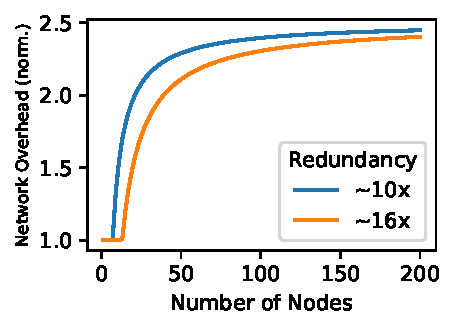
\includegraphics[width=0.6\linewidth]{graphs/network-overhead}
    \caption{The network traffic overhead brought by shard loading.
    The y-axis shows the total network traffic of \sys, normalized to baseline BFT protocols that only transmit transactions and replies.}
    \label{fig:network-overhead}
\end{figure}

We perform numerical analysis to project network traffic under realistic conditions, with a skewed workload that access few shards per transaction.
%The specific plotting equation and the detailed parameters are presented in the appendix.
\lijl{Can summarize these conditions. Are the results workload dependent?}\gd{Done.}
Figure \ref{fig:network-overhead} presents the findings when the system incurs $10\times$ and $16\times$ state size storage.
% The specific plotting equation and parameter values are provided in the appendix.
When the number of nodes is less than the target redundancy, each node effectively stores a complete state copy, and the system exhibits equivalent network traffic to other BFT protocols.
As the node count exceeds the redundancy rate, the system begins to incur network traffic overhead for loading shards; however, this overhead rapidly converges to a constant multiplicative factor relative to the baseline, and the system's network traffic never surpasses $2.5\times$ the baseline traffic.
%This occurs because all BFT protocols must disseminate transactions and reply results to client.
The associated network traffic increases linearly with the number of nodes, as does the network traffic associated with loading shards.
\lijl{Given the fact that normalized traffic converges, can we conclude that network traffic for shard loading also grows linearly?}\gd{I think so.}
Our approach has minimal impact on communication scalability.
